\section{Preliminaries}


The symbols $\le_T$ and
$\equiv_T$ denote polynomial-time Turing reducibility and equivalence.

We use $\mathfrak i$ to denote $\sqrt{-1}$.
We use the matrices
\[
I_2=\begin{bmatrix}1&0\\0&1\end{bmatrix},\quad
N_2=\begin{bmatrix}0&1\\1&0\end{bmatrix},\quad
H=\frac1{\sqrt2}\begin{bmatrix}1&1\\1&-1\end{bmatrix},\quad
K=\frac1{\sqrt2}\begin{bmatrix}1&1\\
\mathfrak i&-\mathfrak i\end{bmatrix}.
\]
The notation $\mathbb{C}^\times$ means $\mathbb{C}\setminus\{0\}$.
For a complex valued matrix $A$, write $A^{\mathtt T}$ for transpose,
$\overline A\,$ for entrywise complex conjugation, and
$A^\dagger=\overline A^{\mathtt T}$ for conjugate transpose.  For row
vectors $\mathbf u,\mathbf v\in\mathbb C^m$, our convention is
\[
\langle\mathbf u,\mathbf v\rangle
=\mathbf u\,\overline{\mathbf v}^{\mathtt T},\qquad
\|\mathbf u\|=\sqrt{\langle\mathbf u,\mathbf u\rangle}.
\]
We also use $|\mathbf u|$ for this norm when no confusion with scalar
absolute value can arise.


\subsection{Definitions and Notations}



A \emph{signature} of arity $n$ is a function
$f:\{0,1\}^n\to\mathbb C$. 
%We also write $\operatorname{arity}(f)=n$ and $f^\alpha=f(\alpha)$.  
%Unless a row orientation is explicitly indicated, the truth table of $f$ is the column vector in lexicographic order.  
For a bit string $\alpha=\alpha_1\cdots\alpha_n$, let $|\alpha|=n$,
\(
\operatorname{wt}(\alpha)=\sum_{j=1}^n\alpha_j,
\)
and denote its bitwise complement by $\overline{\alpha}$.  
The symbols
$0^n=\vec 0^{\,n}$ and $1^n=\vec 1^{\,n}$ denote the all-zero and all-one
strings; the superscript is omitted when its value is clear.  Addition
$\oplus$ of bit strings is coordinatewise over $\mathbb Z_2$.
The \emph{support} of $f$ is
\(
\mathscr S(f)=\{\alpha\in\{0,1\}^n:f(\alpha)\ne0\}.
\)
The signature is zero, written $f\equiv0$, if $\mathscr S(f)=\emptyset$.
A signature is \emph{symmetric} if its value depends only on Hamming weight.
For such a signature of arity $n$, we use the compressed notation
\(
f=[f_0,f_1,\ldots,f_n],
\)
where $f_j$ is the value on every input of weight $j$. 
Let
\(
\Delta_0=[1,0], \,\Delta_1=[0,1].
\)
For $n\ge1$, the equality signature $(=_n)$ is one on $0^n$ and $1^n$ and
zero elsewhere.  The binary disequality signature is
$(\neq_2)=[0,1,0]$. 
More generally, $\neq_{2n}$ denotes the indicator of
\(
x_1= x_2=\ldots= x_n\neq
x_{n+1}=x_{n+2}=\ldots= x_{2n}.
\)
We
write $\mathcal{EQ}=\{=_n\mid n\ge1\}$ and
$\mathcal{DEQ}=\{\neq_{2n}\mid n\ge1\}$.
Also write $\mathcal{EQ}_k=\{=_{nk}\mid n\ge1\}$.
Let
\(
\mathscr E_n=\{\alpha\in\{0,1\}^n:\operatorname{wt}(\alpha)
\text{ is even}\},\,
\mathscr O_n=\{\alpha\in\{0,1\}^n:\operatorname{wt}(\alpha)
\text{ is odd}\}.
\)
A signature has \emph{even parity} or \emph{odd parity} if its support is
contained in $\mathscr E_n$ or $\mathscr O_n$, respectively; it has
\emph{parity} in either case.

We use $=_2^-$ to denote the binary signature $(1, 0, 0, -1)$ and $\neq_2^-$ to denote the binary signature $(0, 1, -1, 0)$.
We may also write $=_2$ as $=_2^+$ and $\neq_2$ as $\neq_2^+$. 
%We use $=_2^{\pm}$ to denote $=_2^+$ or $=_2^-$, and use $\neq_2^{\pm}$ to denote $\neq_2^+$ or $\neq_2^-$.
Let $\mathcal{B}=\{=^+_2, =_2^-, \neq_2^+, \neq_2^-\}$.
We call them Bell signatures which correspond to Bell states $|\Phi^+\rangle=|00\rangle+|11\rangle$, $|\Phi^-\rangle=|00\rangle-|11\rangle$, 
$|\Psi^+\rangle=|01\rangle+|10\rangle$ and 
$|\Psi^-\rangle=|01\rangle-|10\rangle$ in quantum information science \cite{bell1964einstein}.

We use $f_{i_1i_2\ldots i_k}^{a_1a_2\ldots a_k}$ to denote the signature obtained from $f$ by pinning the variables $x_{i_1},x_{i_2},\ldots, x_{i_k}$ to $a_{1},a_2,\ldots, a_k$ respectively.
For example, $f_{i}^a=f(x_1,\ldots,x_{i-1},a,x_{i+1},\ldots,x_n).$
For $S\subseteq[n]$, let $M_S(f)$ be the
$2^{|S|}\times2^{n-|S|}$ matrix whose rows are indexed by assignments
to the variables in $S$ and whose columns are indexed by assignments to
the remaining variables, both in lexicographic order.  We also write
$M_{S,T}(f)$ when the ordered row and column variable lists $S,T$
partition the variables.  In particular,
\[
M_i(f)=
\begin{bmatrix}\mathbf f_i^0\\ \mathbf f_i^1\end{bmatrix},
\qquad
M_{ij}(f)=
\begin{bmatrix}
\mathbf f_{ij}^{00}\\ \mathbf f_{ij}^{01}\\
\mathbf f_{ij}^{10}\\ \mathbf f_{ij}^{11}
\end{bmatrix},
\]\
where $ {\bf {f}}^{a}_{i}$ denotes the row vector indexed by $x_i=a$ in $M_{i}(f)$, and ${\bf {f}}^{ab}_{ij}$ denotes the row vector indexed by $(x_i, x_j)=(a, b)$ in $M_{i j}(f)$.
For a binary signature $b=b(x_1,x_2)$, $M(b)=\left[\begin{smallmatrix}
    b(0,0) & b(0,1)\\
    b(1,0) & b(1,1)
\end{smallmatrix}\right]$ denotes its $2\times2$ signature matrix.




A \emph{signature grid} over $\mathcal F$ is a pair
$\Omega=(G,\pi)$, where $G=(V,E)$ is a graph and $\pi$ assigns to every
$v\in V$ a signature $f_v\in\mathcal F$ of arity $\deg(v)$, and labels the incident edges $E(v)$ at $v$ with input variables of $f_v$.
We consider all 0-1 edge assignments $\sigma$, and each gives an evaluation $\prod_{v\in V}f_v(\sigma|_{E(v)})$, where $\sigma|_{E(v)}$ denotes the restriction of $\sigma$ to $E(v)$.

\begin{definition}[Holant Problems]
The input to the problem $\Holant(\mathcal{F})$ is a signature grid $\Omega=(G,\pi)$ over $\mathcal{F}$.
The output is the partition function
\[
\operatorname{Holant}({\Omega})
=\sum_{\sigma:E(G)\to\{0,1\}}
 \prod_{v\in V}f_v(\sigma|_{E(v)}).
\]
Bipartite Holant problems $\holant{\mathcal{F}}{\mathcal{G}}$
are {Holant} problems
 over bipartite graphs $H = (U,V,E)$,
where each vertex in $U$ or $V$ is labeled by a signature in $\mathcal{F}$ or $\mathcal{G}$ respectively.
When $\{f\}$ is a singleton set, we write $\Holant(\{f\})$ as $\Holant(f)$ and  $\Holant(\{f\}\cup \mathcal{F})$ as $\Holant(f, \mathcal{F}).$ 
\end{definition}

We say a signature $f$ is \emph{realizable} from $\F$, if $\Holant(\F,f)\leq_T \Holant(\F)$.
The \emph{counting constraint satisfaction} problem \#CSP($\mathcal{F}$) is defined as $\Holant(\mathcal{EQ}\mid \mathcal{F}).$
The problem \#$\mathrm{CSP}_k(\mathcal{F})$ is defined as $\holant{\mathcal{EQ}_k}{\mathcal{F}}$.

For a signature $f$ of arity $n$, define its conjugation $\overline{f}$ by $\overline{f}(\alpha)=\overline{f(\alpha)},\,\forall\alpha\in \{0,1\}^n$.
We define the \emph{arrow reversal} of $f$ by
\(
f^{\textsc{ar}}(\alpha)
:=\overline{f(\overline\alpha)},\,\forall\alpha\in \{0,1\}^n.
\)
We say $f$ satisfies \emph{arrow reversal symmetry} (\textsc{ars}) if
$f=f^{\textsc{ar}}$.  
A signature set $\mathcal F$ is
\emph{conjugate closed}, written $\mathcal F=\overline{\mathcal F}$, if
$f\in\mathcal F$ implies $\overline f\in\mathcal F$.  
In this paper, we focus on the case where $\mathcal{F}$ is conjugate closed.
A set $\mathcal G$
is \emph{arrow-reversal closed}, written
$\mathcal G=\mathcal G^{\textsc{ar}}$, if $g\in\mathcal G$ implies
$g^{\textsc{ar}}\in\mathcal G$.  


Let $\mathcal U$ be the set consisting of the binary zero signature and
all binary signatures $b$ for which
\(
M(b)M(b)^\dagger=\lambda I_2
\text{ for some }\lambda>0.
\)
Similarly, $\mathcal O$ consists of the binary zero signature and the
real-valued binary signatures $b$ satisfying
$M(b)M(b)^{\mathtt T}=\lambda I_2$ for some $\lambda>0$.  
%We set $\widehat{\mathcal O}=K^{-1}\mathcal O$ and $\widehat{\mathcal U}=K^{-1}\mathcal U$. 

We use projective binary matrices in the arity-six argument.  For nonzero
matrices $A,B$, write $A\sim B$ if $A=\lambda B$ for some
$\lambda\in\mathbb C^\times$, and let $[A]$ denote the projective class.
Set
\[
X=N_2,\qquad
Y=\begin{bmatrix}0&-\mathfrak i\\ \mathfrak i&0\end{bmatrix},\qquad
Z=\begin{bmatrix}1&0\\0&-1\end{bmatrix},\qquad
J=\mathfrak iY=\begin{bmatrix}0&1\\-1&0\end{bmatrix}.
\]
Notice that $I_2,X,Z,J$ are matrices of the signatures $=_2^{+},\neq_2^{+},=_2^{-},\neq_2^{-}$, respectively.
For $\varepsilon_1,\varepsilon_2,\varepsilon_3\in\{\pm1\}$, put
\[
C_{\varepsilon_1,\varepsilon_2,\varepsilon_3}
=\frac12\bigl(I_2+\varepsilon_1\mathfrak iX
                 +\varepsilon_2J+\varepsilon_3\mathfrak iZ\bigr).
\]
The projective tetrahedral group and its normal Klein-four subgroup are
\[
\Gamma
=\{[I_2],[X],[Z],[J]\}
 \cup
 \{[C_{\varepsilon_1,\varepsilon_2,\varepsilon_3}]:
        \varepsilon_1,\varepsilon_2,\varepsilon_3\in\{\pm1\}\},
\qquad
K_4=\{[I_2],[X],[Z],[J]\}.
\]
Thus $\Gamma\cong A_4$ and $K_4\cong V_4$, where $A_4$ is the alternating group of order 12 and $V_4$ is the Klein group.
We suppress the projective
brackets when a displayed unitary representative is intended. 
In this paragraph, and everywhere in the quantum arguments, $Z$ is the Pauli
matrix rather than a holographic transformation.


\subsection{Holographic Transformation}
To introduce the idea of holographic transformation,
it is convenient to consider bipartite graphs.
For a general graph,
we can always transform it into a bipartite graph while preserving the Holant value,
as follows.
For each edge in the graph,
we replace it by a path of length two.
(This operation is called the \emph{2-stretch} of the graph and yields the edge-vertex incidence graph.)
Each new vertex is assigned the binary \textsc{Equality} signature $=_2$. Thus, we have $\holant{=_2}{\mathcal{F}}\equiv_T \Holant(\mathcal{F})$.


For an invertible $2$-by-$2$ matrix $T \in {\bf GL}_2({\mathbb{C}})$
 and a signature $f$ of arity $n$, written as
a column vector (covariant tensor) $f \in \mathbb{C}^{2^n}$, we denote by
$Tf = T^{\otimes n} f$ the transformed signature.
  For a signature set $\mathcal{F}$,
define $T\mathcal{F} = \{T f \mid  f \in \mathcal{F}\}$ the set of
transformed signatures.
For signatures written as
 row vectors (contravariant tensors) we define
$f T^{-1}$ and  $\mathcal{F} T^{-1}$ similarly.
Whenever we write $T f$ or $T \mathcal{F}$,
we view the signatures as column vectors;
similarly for $f T^{-1}$ or $\mathcal{F} T^{-1}$ as row vectors.
We can also represent $Tf$ as the matrix $M_{S_k}(Tf)$ with the assignments of variables in $S_k$ as row index and the assignments of the other $n-k$ variables as column index. 
Then,  we  have $M_{S_k}(Tf)=T^{\otimes k}M_{S_k}(f)(T^{\tt T})^{\otimes n-k}$. Similarly, $M_{S_k}(fT^{-1})=({T^{-1}}^{\tt T})^{\otimes k}M_{S_k}(f)(T^{-1})^{\otimes n-k}$.
%In the special case of the Hadamard matrix
%$H_2 = \frac{1}{\sqrt{2}} \left[\begin{smallmatrix} 1 & 1 \\ 1 & -1 \end{smallmatrix}\right]$,
%we also define $\widehat{\mathcal{F}} = H_2  \mathcal{F}$.
%Note that $H_2$ is orthogonal.
%Since constant factors are immaterial, for convenience we sometime
%drop the factor $\frac{1}{\sqrt{2}}$ when using $H_2$. 

Let $T \in {\bf GL}_2({\mathbb{C}})$.
The holographic transformation defined by $T$ is the following operation:
given a signature grid $\Omega = (H, \pi)$ of $\holant{\mathcal{F}}{\mathcal{G}}$,
for the same bipartite graph $H$,
we get a new signature grid $\Omega' = (H, \pi')$ of $\holant{\mathcal{F} T^{-1}}{T \mathcal{G}}$ by replacing each signature in
$\mathcal{F}$ or $\mathcal{G}$ with the corresponding signature in $\mathcal{F} T^{-1}$ or $T \mathcal{G}$.

\begin{theorem}[\cite{Valiant08}]\label{thm: holographic transformation}
 For every $T \in {\bf GL}_2({\mathbb{C}})$,
  $\Holant(\mathcal{F} \mid \mathcal{G}) \equiv_T \Holant(\mathcal{F} T^{-1} \mid T \mathcal{G}).$
\end{theorem}

Therefore,
a holographic transformation does not change the complexity of the Holant problem in the bipartite setting. 
A particular useful holographic transformation is the $K$-transformation.
Direct calculation shows $(=_2)K=(\neq_2)$, so
\(
\holant{=_2}{\mathcal F}
\equiv_T
\holant{\neq_2}{K^{-1}\mathcal F}.
\)
Accordingly, throughout this paper
\[
\widehat f:=K^{-1}f,
\qquad
\widehat{\mathcal F}:=K^{-1}\mathcal F.
\]
We also call
$\holant{\neq_2}{\widehat{\mathcal F}}$ the
{$K$-Holant} formulation of $\Holant(\mathcal F)$.


\begin{lemma}\label{lm: conjugation and K-trans}
Let $f$ be a complex-valued signature of arity $n$.  For every
$\alpha\in\{0,1\}^n$,
\(
\widehat{\overline f}(\alpha)
=\overline{\widehat f(\overline\alpha)}.
\)
\end{lemma}
\begin{proof}
Using $K^{\mathtt T}=N_2K^{-1}$, we have
\(
\widehat{\overline f}
=(K^{-1})^{\otimes n}\overline f
=\overline{(K^{\mathtt T})^{\otimes n}f}
=N_2^{\otimes n}\overline{\widehat f},
\)
which is the stated entrywise identity.
\end{proof}

The preceding lemma immediately gives
the following equivalence.
\begin{lemma}\label{lm: conjugate closed and ars closed}
$\mathcal F$ is conjugate closed if and only if
$\widehat{\mathcal F}$ is arrow-reversal closed.
\end{lemma}



\subsection{Signature Factorization}

For signatures $f$ and $g$ on disjoint variable sets $\{x_1,\ldots,x_n\}$ and $\{y_1,\ldots,y_m\}$, $f\otimes g$ denotes their tensor product, with $(f\otimes g)(x_1,\ldots, x_n,y_1,\ldots,y_m)=f(x_1,\ldots,x_n)\cdot g(y_1,\ldots, y_m)$.
Recall that by our definition, every signature has arity at least one.
A nonzero signature $g$ \emph{divides} $f$ denoted by $g \mid f$, if there is a signature $h$ such that  $f=g \otimes h$
%=h \otimes g$ 
%%% the permutation includes this other order
(with possibly a permutation of variables) or there is a constant $\lambda$ such that $f= \lambda \cdot g$.
In the latter case, if $\lambda \neq 0$, then we also have $f \mid g$ since $g= \frac{1}{\lambda} \cdot f$.
%When $h$ is a nonzero signature of arity $0$, i.e. a  constant $c \not = 0$,
%it is a \emph{unit} and $g \otimes h$ is just $cg$. 
For nonzero signatures, if both $g\mid f$ and $f \mid g$, then they are nonzero constant multiples of
each other, and 
we say $g$ is an \emph{associate} of $f$, 
denoted by $g \sim f$.
In terms of  this division relation,
the notions of \emph{irreducible}  signatures  and \emph{prime} signatures have been defined.
They are proved equivalent and thus, the \emph{unique prime factorization} (UPF) of signatures is established \cite{cai-fu-shao-eo}.

%\begin{definition}
%A signature $f$ is irreducible (a prime signature) if it cannot be decomposed 
%\end{definition}
A nonzero signature $f$ is irreducible  if there are no signatures $g$ and $h$ such that $f=g\otimes h$. 
A nonzero signature $f$ is a prime signature
if $f \mid g\otimes h$
implies that $f \mid g$ or $f \mid h$.  These notions
are equivalent.
%On the contrary, 
We say a signature $f$ is reducible  if $f = g \otimes h$,
for some signatures $g$ and $h$. All zero signatures 
of arity greater than 1 are reducible.
A prime factorization of a signature $f$ is $f=g_1\otimes \ldots \otimes g_k$ up to a permutation of
variables, where each $g_i$ is irreducible. 
%%% 0 is reducible
% unit , arity-0 nonzero constant is neither
% arity 1 nonzero is irre
% nonzero arity >= 2 : reducible if there is a decomp 
% of f = lower arity g \otimes lower arity  h
% and irre otherwise.


\begin{lemma}[Unique prime factorization~\cite{cai-fu-shao-eo}]\label{unique}
Every nonzero signature $f$ has a prime factorization.
If  $f$ has  prime factorizations
 $f=g_1\otimes \ldots \otimes g_k$ and $f=h_1\otimes \ldots \otimes h_\ell$,
both up to a permutation of variables,
then $k=\ell$ and after reordering the factors we have $g_i \sim h_i$  for all $i$. 
%where $\lambda_i$ are nonzero constants.
\end{lemma}

For $k\ge1$, let
\[
\mathcal F^{\otimes k}
=\left\{\lambda\bigotimes_{j=1}^k f_j:
  \lambda\in\mathbb C^\times,\ f_j\in\mathcal F\right\},\qquad
\mathcal F^\otimes=\bigcup_{k\ge1}\mathcal F^{\otimes k}.
\]
We also write $\langle\mathcal F\rangle$ for this normalized tensor
closure.

\begin{lemma}[\cite{Lin_Wang_Decomposition_lemma} Lemma 3.1]\label{lm: decomposition of tensor power}
    Let $\F$ be a set of signatures. Then
    $$
        \Holant(\F,f)\leq_T \Holant(\F,f^{\otimes d}),
    $$
    for all $d\geq 1$.
\end{lemma}


\subsection{Gadget Construction}

An \emph{$\mathcal F$-gate} is a finite signature grid over $\mathcal F$
with some dangling edges; summing over its internal edges realizes the
signature on the dangling edges. 
%We say a signature $f$ is \emph{realizable} from $\F$, if $\Holant(\F,f)\leq_T \Holant(\F)$.
It is clear that if $f$ is the signature of an $\mathcal F$-gate, it is realizable from $\mathcal{F}.$
In the following we do not distinguish an $\mathcal{F}$-gate and its signature.

We record some frequently used gadgets in this paper. 
The following four basic constructions are illustrated in \cref{fig:gadget-constructions}.

\paragraph{Merging}
Given a binary signature $b$ and a signature $f$ with distinct variables $x_i,x_j$, the signature obtained \emph{merging} (or \emph{contracting}) variables $x_i,x_j$ of $f$ using $b$ is the following signature
\[
(\partial_{ij}^b f)(x_{[n]\setminus\{i,j\}})
=\sum_{a,c\in\{0,1\}}b(a,c)
  f(x_1,\ldots,x_{i-1},a,x_{i+1},\ldots,x_{j-1},c,x_{j+1},\ldots,x_n).
\]
When $b$ is $=_2$, we simply say merge $x_i$ and $x_j$ of $f$. 
We abbreviate
$\partial_{ij}f:=\partial_{ij}^{=_2}f=f_{ij}^{00}+f_{ij}^{11}$.
We also use the notation $\partial^{M(b)}_{ij}f$ for $\partial^{b}_{ij}f$, where $M(b)$ is the $2$ by 2 signature matrix of $b$.
We use $\partial_{(i_1j_1)\ldots(i_kj_k)}f$ to denote $\partial_{i_1j_1}\ldots\partial_{i_kj_k}f$ for short.
It is clear that the operators $\partial_{ij}$ and $\partial_{k\ell}$ commute if $\{i,j\}\cap \{k,\ell\}=\emptyset.$
For a signature class $\mathscr C$, the notation
$f\in\int\mathscr C$ means that
$\partial_{ij}f\in\mathscr C$ for every pair $i\ne j$.

\paragraph{Binary extension}
    Given a binary signature $b(x_1,x_2)$ and an arity-$n$ signature $f(y_1,\ldots, y_n)$, we may connect $x_i$ of $b$ to $y_j$ of $f$, and obtain a new signature.
    This is called a \emph{binary extension} or \emph{binary modification} to $f$.



\begin{lemma}\label{lem-binary-sim}
    Let ${b_1}(x_1, y_1), {b_2}(x_2, y_2)\in {\mathcal{U}}$. 
    If by connecting the variable $x_1$ of ${b_1}$ and the variable $x_2$ of ${b_2}$ using $=_2$, we get $\lambda\cdot (=_2)(y_1, y_2)$ for some $\lambda\in \mathbb{C}^\times$, then ${b_1}\sim \overline{b_2}$. 
    Moreover, by connecting the variable $y_1$ of ${b_1}$ and the variable $y_2$ of ${b_2}$, we will get $\lambda\cdot (=_2)(x_1, x_2)$.
\end{lemma}

\begin{proof}
Clearly both $b_1$ and $b_2$ are non-zero, otherwise connecting them we obtain a zero signature.
Since $b_1, b_2\in \mathcal{U}$ and they are non-zero, there exists $\lambda_1,\lambda_2\in \mathbb C^\times$ such that $M(b_1)M(b_1)^\dagger=\lambda_1I_2$ and  $M(b_2)M(b_2)^\dagger=\lambda_2I_2$.
%Consider matrices $M_1(b_1)=M^{\tt T}_2(b_1)$ and $M_1(b_2)=M^{\tt T}_2(b_2)$.
By connecting $x_1$ of $b_1$ and $x_2$ of $b_2$, we obtain the binary signature $b_3(y_1,y_2)$ with matrix $M(b_3)=M(b_1)^{\tt T}M(b_2)=\lambda I_2$ for some $\lambda\in \mathbb{C}^\times.$
So $M(b_2)=\lambda (M(b_1)^{\tt T})^{-1}=\frac{\lambda}{\lambda_1} \overline{M(b_1)}$.
Hence $b_1\sim \overline{b_2}$.
Also, by connecting the variable $y_1$ of ${b_1}$ and the variable $y_2$ of ${b_2}$, we will get the signature $b_4(x_1,x_2)$ with matrix $M(b_4)=M(b_1)M(b_2)^{\tt T}=M(b_1)\cdot \frac{\lambda}{\lambda_1}M(b_1)^\dagger=\lambda\cdot(=_2)(x_1, x_2).$
\end{proof}

\paragraph{Mating and first order orthogonality}
Given a (complex-valued) signature $f$ of arity $n\geqslant 2$, we connect $f$ and $\overline{f}$ in the following manner:
Fix a set $S$ of $n-m$ variables among all $n$ variables of $f$. 
For each $x_k\in S$, connect $x_k$ of $f$ with the corresponding variable $x_k$ of $\overline{f}$ using $=_2$. 
The variables that are not in $S$ are called dangling variables.
%In this paper, we only consider the case that $m=1$ or $2$.
For $m=1$, there is one dangling variable $x_i$. Then, 
the mating construction  realizes a binary signature, denoted by $\mathfrak m_{i}f$.
\begin{figure}[t]
\centering
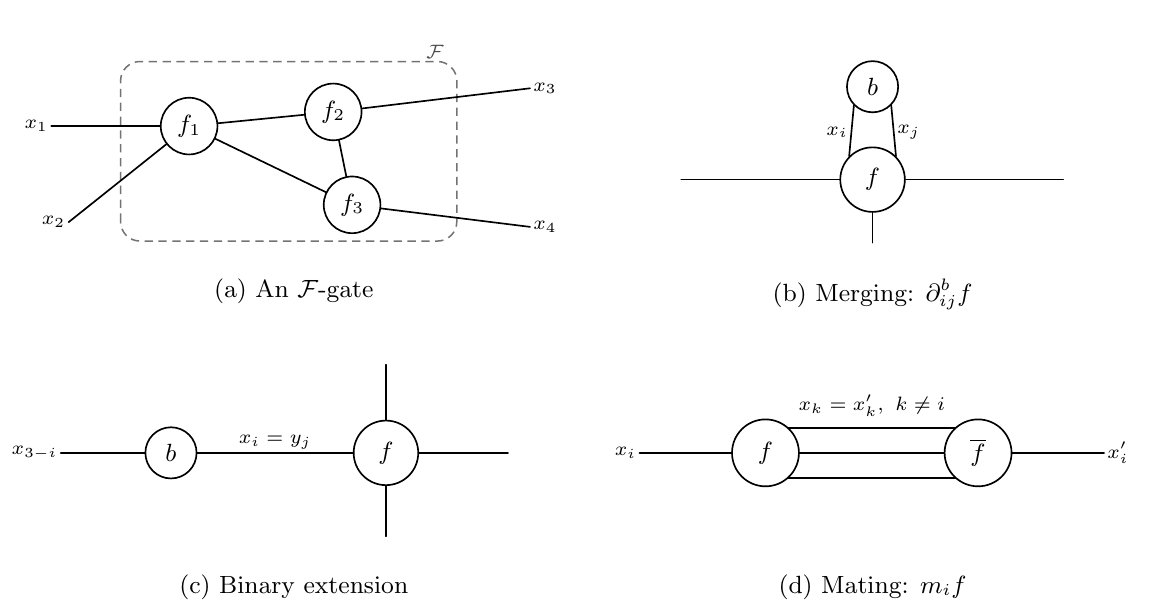
\begin{tikzpicture}[
    wire/.style={draw=black, line width=0.6pt, line cap=round},
    boundary/.style={draw=black!55, densely dashed, line width=0.55pt,
        rounded corners=7pt},
    signature/.style={draw=black, circle, fill=white, minimum size=7.2mm,
        inner sep=0pt, line width=0.6pt, font=\small},
    small signature/.style={signature, minimum size=6.5mm},
    port label/.style={font=\scriptsize, inner sep=1pt},
    panel label/.style={font=\small, anchor=north}
]

% (a) An F-gate
\begin{scope}[shift={(0,3.75)}]
    \path[use as bounding box] (0,0) rectangle (6.75,3.35);

    \draw[boundary] (1.18,0.64) rectangle (5.45,2.92);
    \node[port label, anchor=south east, text=black!70]
        at (5.33,2.92) {$\mathcal F$};

    \draw[wire] (0.30,2.10) -- (2.05,2.10);
    \draw[wire] (0.52,0.88) -- (2.05,2.10);
    \draw[wire] (2.05,2.10) -- (3.88,2.28);
    \draw[wire] (2.05,2.10) -- (4.12,1.10);
    \draw[wire] (3.88,2.28) -- (4.12,1.10);
    \draw[wire] (3.88,2.28) -- (6.38,2.58);
    \draw[wire] (4.12,1.10) -- (6.38,0.82);

    \node[signature] at (2.05,2.10) {$f_1$};
    \node[signature] at (3.88,2.28) {$f_2$};
    \node[signature] at (4.12,1.10) {$f_3$};

    \node[port label, left] at (0.30,2.10) {$x_1$};
    \node[port label, left] at (0.52,0.88) {$x_2$};
    \node[port label, right] at (6.38,2.58) {$x_3$};
    \node[port label, right] at (6.38,0.82) {$x_4$};
    \node[panel label] at (3.38,0.28)
        {\textup{(a)} An $\mathcal F$-gate};
\end{scope}

% (b) Merging two variables of f using b
\begin{scope}[shift={(7.35,3.75)}]
    \path[use as bounding box] (0,0) rectangle (6.75,3.35);

    \node[small signature] (merge-b) at (3.38,2.60) {$b$};
    \node[signature, minimum size=8.2mm] (merge-f) at (3.38,1.42) {$f$};

    \draw[wire] (merge-b.225) --
        node[port label, left, pos=0.53] {$x_i$} (merge-f.135);
    \draw[wire] (merge-b.315) --
        node[port label, right, pos=0.53] {$x_j$} (merge-f.45);
    \draw[wire] (0.95,1.42) -- (merge-f.180);
    \draw[wire] (merge-f.0) -- (5.80,1.42);
    \draw[wire] (3.38,0.62) -- (merge-f.270);

    \node[panel label] at (3.38,0.28)
        {\textup{(b)} Merging: $\partial_{ij}^{b}f$};
\end{scope}

% (c) Binary extension
\begin{scope}
    \path[use as bounding box] (0,0) rectangle (6.75,3.35);

    \node[small signature] (ext-b) at (1.82,1.70) {$b$};
    \node[signature, minimum size=8.2mm] (ext-f) at (4.55,1.70) {$f$};

    \draw[wire] (0.42,1.70) -- (ext-b.180);
    \draw[wire] (ext-b.0) --
        node[port label, above] {$x_i=y_j$} (ext-f.180);
    \draw[wire] (ext-f.0) -- (6.10,1.70);
    \draw[wire] (4.55,2.82) -- (ext-f.90);
    \draw[wire] (4.55,0.64) -- (ext-f.270);

    \node[port label, left] at (0.42,1.70) {$x_{3-i}$};
    \node[panel label] at (3.38,0.28)
        {\textup{(c)} Binary extension};
\end{scope}

% (d) Mating f with its conjugate
\begin{scope}[shift={(7.35,0)}]
    \path[use as bounding box] (0,0) rectangle (6.75,3.35);

    \draw[wire] (0.42,1.70) -- (2.02,1.70);
    \draw[wire] (2.02,2.02) -- (4.72,2.02);
    \draw[wire] (2.02,1.70) -- (4.72,1.70);
    \draw[wire] (2.02,1.38) -- (4.72,1.38);
    \draw[wire] (4.72,1.70) -- (6.32,1.70);

    \node[signature, minimum size=8.5mm] at (2.02,1.70) {$f$};
    \node[signature, minimum size=8.5mm] at (4.72,1.70) {$\overline f$};

    \node[port label, left] at (0.42,1.70) {$x_i$};
    \node[port label, right] at (6.32,1.70) {$x_i'$};
    \node[port label, fill=white] at (3.37,2.30)
        {$x_k=x_k',\ k\ne i$};
    \node[panel label] at (3.38,0.28)
        {\textup{(d)} Mating: $\mathfrak m_i f$};
\end{scope}

\end{tikzpicture}
\caption{Basic gadget constructions.
\textup{(a)} An $\mathcal F$-gate, with every internal signature in
$\mathcal F$.
\textup{(b)} Merging the variables $x_i$ and $x_j$ of $f$ with the binary
signature $b$, producing $\partial_{ij}^{b}f$.
\textup{(c)} A binary extension formed by identifying $x_i$ of $b$ with
$y_j$ of $f$.
\textup{(d)} Mating $f$ with $\overline f$ on all variables except $x_i$,
producing $\mathfrak m_i f$; the three parallel wires represent these
$n-1$ contractions.
Joined half-edges are contracted, whereas unjoined half-edges are free
variables.}
\label{fig:gadget-constructions}
\end{figure}

It can be represented by matrix multiplication. 
We have 
\begin{equation}\label{m-form}
M(\mathfrak m_{i}f)=M_{i}(f)I_2^{\otimes (n-1)}M^{\tt T}_{i}(\overline{f})=M_i(f)M_i(f)^{\dagger}
=\begin{bmatrix}
{\bf {f}}^{0}_i\\
{\bf {f}}^{1}_i\\
\end{bmatrix}
\left[\begin{matrix}
{{\bf {\overline{f}}}^{0}_i}^{\tt T} &{{\bf {\overline{f}}}^{1}_i}^{\tt T}\\
\end{matrix}\right]
=\left[\begin{matrix}
|{\bf f}_i^0|^2 &  \langle {\bf f}_i^0, {\bf f}_i^1 \rangle\\
\langle {\bf f}_i^1, {\bf f}_i^0 \rangle & |{\bf f}_i^1|^2\\
\end{matrix}\right],
\end{equation}
where $\langle \cdot, \cdot\rangle$ denotes the 
inner product and $|\cdot|$ denotes the  norm defined by this inner product.
Note that $\langle{\bf f}^{0}_i, {\bf f}^{1}_i\rangle=\overline{\langle{\bf f}^{1}_i, {\bf f}^{0}_i\rangle}$ and $|\langle{\bf f}^{0}_i, {\bf f}^{1}_i\rangle|\leqslant|{\bf f}^{0}_i||{\bf f}^{1}_i|$ by the Cauchy-Schwarz inequality.

\begin{definition}[First order orthogonality \cite{odd_holant_real}]\label{def-first-order}
       Let $f$ be a complex-valued signature of arity $n \geqslant 2$. It satisfies the \emph{first order orthogonality}, denoted by $f\in$ {\sc 1st-Orth}, if there exists some $\mu\neq 0$ such that for all indices $i\in [n]$, the entries of $f$ satisfy the following equations
\begin{equation*}
    |{\bf f}_{i}^{0}|^2=|{\bf f}_{i}^{1}|^2=\mu, \text{ and } \langle{\bf f}_{i}^{0}, {\bf f}_{i}^{1}\rangle =0.
\end{equation*}
    \end{definition}
    
\begin{proposition}\label{prop: invariant 1st-Orth}
    {\sc 1st-Orth} is invariant up to conjugation and holographic transformation by $T\in \mathbf{U}_2(\mathbb{C})$.
\end{proposition}

\begin{proof}
    Suppose $f$ has arity $n$.
    Clearly $f\in$ {\sc 1st-Orth} $\iff $ $\overline{f}\in$ {\sc 1st-Orth}.
    Now take $T\in \mathbf{U}_2(\mathbb{C})$, we have
    \begin{equation*}
        \begin{aligned}
            M(\mathfrak m_i (Tf))
            =&M_i(Tf)M_i(Tf)^{\dagger}\\
            =&TM_i(f)(T^{\tt T})^{\otimes n-1}\overline{T}^{\otimes n-1}M_i(f)^\dagger T^\dagger\\
            =&TM_i(f)M_i(f)^\dagger T^\dagger\\
            =&TM(\mathfrak m_i f)T^\dagger.\\
        \end{aligned}
    \end{equation*}
    So, for every $\mu>0$, $M(\mathfrak m_i f)=\mu I_2 \iff M(\mathfrak m_i (Tf))=\mu I_2$.
    That is, $f\in$ {\sc 1st-Orth} $\iff $ $Tf\in$ {\sc 1st-Orth}.
\end{proof}

\begin{remark}
    Since $K\in \mathbf{U}_2(\mathbb{C})$, $f\in$ {\sc 1st-Orth} $\iff \widehat{f}\in $ {\sc 1st-Orth}.
\end{remark}

\iffalse
Similarly, in the setting of $\holant{\neq_2}{\widehat{\mathcal{F}}}$, the above mating operation is equivalent to connecting variables in $S$ of $\widehat{f}$ and those of $\widehat{\overline{f}}$ using $\neq_2$. 
We denote the resulting signature by  $\widehat{\mathfrak{m}}_i\widehat{f}$.
It is easy to check that $\widehat{\mathfrak{m}}_i\widehat{f}=\widehat{{\mathfrak{m}}_i{f}}.$
So $f\in$ {\sc 1st-Orth} $\iff \exists \mu>0,M(\mathfrak m_if)=\mu I_2\iff  \exists \mu>0, M(\widehat{\mathfrak m}_i \widehat{f})= \mu N_2$.
We can also calculate the matrix $M(\widehat{\mathfrak m}_i\widehat{f})$ specifically as follows:
\begin{equation*}
    M(\widehat{\mathfrak{m}}_i\widehat{f})=
    M_{i}(\widehat f)N_2^{\otimes n-1}M^{\tt T}_{i}\left(\widehat{\overline{f}}\right)=
    \left[\begin{matrix}
    \widehat{{\bf f}}_i^0\\
    \widehat{{\bf f}}_i^1
    \end{matrix}\right]
    \left[\begin{matrix}
    0 & 1 \\
     1 & 0
    \end{matrix}\right]^{\otimes (n-1)}
    \left[\begin{matrix}
    {\widehat{\overline{{\bf f}_i^{0}}}}^{\tt T} & {\widehat{\overline{{\bf f}_i^{1}}}^{\tt T}}
    \end{matrix}\right].\\
\end{equation*}
By \cref{lm: conjugation and K-trans},
we have
\begin{equation*}
    N_2^{\otimes (n-1)}{\widehat{\overline{{\bf f}_i^{0}}}^{\tt T}}
    =N_2^{\otimes (n-1)}[\overline{\widehat f^{1,11\ldots1}}, \overline{\widehat f^{1, 11\ldots0}}, \ldots, \overline{\widehat f^{1, 00\ldots0}}]^{\tt T}\\=[\overline{\widehat f^{1,00\ldots0}}, \overline{\widehat f^{1,00\ldots1}}, \ldots, \overline{\widehat f^{1, 11\ldots1}}]^{\tt T}={\overline{\widehat{{\bf f}}_i^{1}}}^{\tt T}.
\end{equation*}
Thus, we have
\begin{equation}\label{eqn: 1st-Orth by neq}
M(\widehat{\mathfrak{m}}_i\widehat{f})=
\left[\begin{matrix}
\widehat{{\bf f}}_i^0\\
\widehat{{\bf f}}_i^1
\end{matrix}\right]
\left[\begin{matrix}
0 & 1 \\
 1 & 0
\end{matrix}\right]^{\otimes (n-1)}
\left[\begin{matrix}
    {\widehat{\overline{{\bf f}_i^{0}}}}^{\tt T} & {\widehat{\overline{{\bf f}_i^{1}}}^{\tt T}}
    \end{matrix}\right]\\
=\left[\begin{matrix}
\widehat{{\bf f}}_i^0\\
\widehat{{\bf f}}_i^1
\end{matrix}\right]
\left[\begin{matrix}
{\overline{\widehat{{\bf f}}_i^{1}}}^{\tt T} &\overline{{\widehat{{\bf f}}_i^{0}}}^{\tt T}
\end{matrix}\right]
=\left[\begin{matrix}
\langle \widehat{{\bf f}}_i^0, \widehat{{\bf f}}_i^1 \rangle & |\widehat{{\bf f}}_i^0|^2\\
|\widehat{{\bf f}}_i^1|^2 & \langle \widehat{{\bf f}}_i^1, \widehat{{\bf f}}_i^0 \rangle
\end{matrix}\right].
\end{equation}
\cref{eqn: 1st-Orth by neq} combined with \cref{prop: invariant 1st-Orth} also shows that $\exists \mu>0,M(\mathfrak m_if)=\mu I_2$ iff $ \exists \mu>0, M(\widehat{\mathfrak m}_i \widehat{f})= \mu N_2$.
\fi

\begin{lemma}\label{lm: 1st-Orth uniform}
    Let $f$ be a signature of arity $n$.
    If for all indices $i\in [n]$, $M(\mathfrak{m}_{i}f)= \mu_i I_2$ for some real $\mu_i\neq 0$, then $f$ satisfies {\sc 1st-Orth} (i.e., all $\mu_i$ have the same value).
\end{lemma}
\begin{proof}
    For an arbitrary $i\in[n]$, connecting two variables of $\mathfrak m_if$ by $=_2$, we will get Holant value $2\mu_i\neq 0.$
    On the other hand, this value is equal to $\sum_{\alpha\in\{0,1\}^n}f(\alpha)\overline{f(\alpha)}$ which is independent of $i$.
    Therefore, all $\mu_i$ have the same value.
\end{proof}

\begin{lemma}\label{lm: not 1st-orth is hard}
    Let $\mathcal{F}$ be a conjugate closed set of signatures containing a nonzero signature that does not satisfy {\sc 1st-Orth}. 
    If $\mathcal{F}$ does not satisfy condition \rm{(\ref{cond: tractable classes})},
    then $\Holant(\mathcal{F})$ is \#P-hard.
\end{lemma}
 
\begin{proof}
    Let $f\in\F$ be a nonzero signature that does not satisfy {\sc 1st-Orth}, and consider $M_{i}(f)$ for an arbitrary index $i$.
    Clearly, $M(\mathfrak{m}_if)=M_{i}(f)M^\dagger_{i}(f)$ is a Hermitian positive semi-definite matrix, which is diagonalizable with two non-negative real eigenvalues $\lambda_i\geqslant\mu_i\geqslant 0$.
    These two eigenvalues are not both zero since $f \not\equiv 0$, and so $M(\mathfrak{m}_if)\neq 0$. Thus, $\lambda_i\neq 0$.
    Then, $|\frac{\mu_i}{\lambda_i}|=1$ iff $\lambda_i=\mu_i$. 
    %In other words, $M(\mathfrak{m}_if)= \mu_i I_2$ for some real $\mu_i\neq 0$.

    Since $f$ does not satisfy {\sc 1st-Orth}, by \cref{lm: 1st-Orth uniform}, there is an index $i$ such that $M(\mathfrak{m}_if)\neq  \mu_i I_2$ for any real $\mu_i\neq 0$. 
    Thus, $M(\mathfrak{m}_if)$ has two eigenvalues with different norms. 
    By \cref{lm: 2 by 2 interpolation}, we can realize a nonzero binary signature $g$ such that $M(g)$ is degenerate. This implies that  $g$ can be factorized as a tensor product of two nonzero unary signatures. 
    By \cref{lm: decomposition}, we can realize a nonzero unary signature.
    By \cref{lm: odd holant with conjugation}, $\Holant(\mathcal{F})$ is \#P-hard.
\end{proof}

\subsection{Tractable Signatures}\label{subsec: tractable signatures}

We give some known signature sets that define polynomial time computable (tractable) counting problems.


\begin{definition}
    The class $\mathscr T$ consists of all signatures that, up to a
    permutation of variables, are tensor products of unary and binary signatures.
\end{definition}


\begin{definition}[Affine signatures]\label{def: affine}
A signature $f(x_1,\ldots,x_n)$ is \emph{affine} if it has the form
\[
f(x_1,\ldots,x_n)
=\lambda\,\chi_{A\mathbf x=0}\,
 \mathfrak i^{\,Q(x_1,\ldots,x_n)},
\]
where $\lambda\in\mathbb C$,
$\mathbf x=(x_1,\ldots,x_n,1)^{\mathsf T}$, $A$ is a matrix over
$\mathbb Z_2$, and $Q\in\mathbb Z_4[x_1,\ldots,x_n]$ is multi-linear polynomial of
degree at most two with even mixed coefficients.  
Equivalently,
\[
Q(x_1,\ldots,x_n)
=a_0+\sum_{k=1}^n a_kx_k
 +\sum_{1\le i<j\le n}2b_{ij}x_ix_j,
\qquad a_k,b_{ij}\in\mathbb Z_4.
\]
The equation $A\mathbf x=0$ is evaluated over $\mathbb Z_2$, and $\chi$ is a 0-1 indicator function such that $\chi_{A\mathbf{x}=0}$ is 1 iff $A\mathbf{x}=0.$
The class of affine signatures is denoted by $\mathscr A$. 
\end{definition}

We say that
$f$ has \emph{affine support} if $\mathscr S(f)$ is an affine subspace of
$\mathbb Z_2^n$.
Clearly, any affine signature has affine support. 
%Moreover, we have that any signature of product type has affine support \cite{jcbook}.

\begin{lemma}\label{lm: affine singular value}
    Let $f\in \mathscr{A}$ be a signature of arity n.
    For every subset of indices $S\subseteq[n]$, the nonzero rows of the $2^{|S|}$ by $2^{n-|S|}$ matrix $M_{S,\overline{S}}(f)$ are either orthogonal or proportional.
    Moreover, the $2^{|S|}$ by $2^{n-|S|}$ matrix $M_{S,\overline{S}}(f)$ has equal non-zero singular values, and $\mathrm{rank}(M_{S,\overline{S}}(f))$ is the power of 2.
\end{lemma}

\begin{proof}
    By the definition of affine signature, it has normal form $f(\mathbf{x})=\lambda \mathbf{1}_{A\mathbf{x}=b}\mathfrak{i}^{Q(\mathbf{x})}$, where the solution set of $A\mathbf x=b$ over $\mathbb Z_2$ is an affine subspace over $\mathbb Z_2^n$ and the $Q(\mathbf{x})$ is a multi-linear polynomial of degree at most two with even mixed coefficients.

    For any subset $S\subseteq [n]$, let $\mathbf{x}=(\mathbf{x}_S,\mathbf{x}_{\overline{S}})$ and  $\mathbf{x}_S,\mathbf{x}_{\overline{S}}$ be the vector of variables in $S$ and $\overline{S}$ respectively. Thus, the signature matrix $M_{S,\overline{S}}(f)$ has row index $\mathbf{x}_S$ and column index $\mathbf{x}_{\overline{S}}$. Since the support of $f$ is an affine subspace, we can assume that $\mathscr{S}(f)=L+(\mathbf{x}_S',\mathbf{x}_{\overline{S}}')$ where $L$ is the solution set of $A\mathbf{x}=0$ over $\mathbb Z_2$, hence $L$ is an linear subspace over $\mathbb{Z}_2^n$, and $(\mathbf{x}_S',\mathbf{x}_{\overline{S}}')$ is a special solution of $A\mathbf{x}=b$.

    Let $W:= \{\mathbf{u}_S\in \{0,1\}^{|S|}: \exists \mathbf{v}_{\overline{S}},(\mathbf{u}_S,\mathbf{v}_{\overline{S}})\in L\}$. This $W$ help us to give the set of all row indices of all nonzero rows, which is the set $\mathbf{x}_S+W$. Let $V:= \{\mathbf{v}_{\overline{S}}\in \{0,1\}^{|\overline{S}|}:(\mathbf{0},\mathbf{v}_{\overline{S}})\in L\}$. This $V$ help us to give the set of column indices that the entry of the matrix is nonzero when giving a nonzero row index. Giving an index $\mathbf{x}_S^{(1)}$ of a nonzero row, there must exist a index $\mathbf{x}_{\overline{S}}^{(1)}$ such that $(\mathbf{x}_S^{(1)},\mathbf{x}_{\overline{S}}^{(1)})\in L+(\mathbf{x}_S',\mathbf{x}_{\overline{S}}')$ since the row is not all zero. Then the index of column that the entry is nonzero belongs to $\mathbf{x}_{\overline{S}}^{(1)}+V$, since for any $\mathbf{v}_{\overline{S}}\in V$, we have $(\mathbf{x}_S^{(1)},\mathbf{x}_{\overline{S}}^{(1)}+\mathbf{v}_{\overline{S}})=(\mathbf{x}_S^{(1)},\mathbf{x}_{\overline{S}}^{(1)})+(\mathbf{0},\mathbf{v}_{\overline{S}})\in L+(\mathbf{x}_S',\mathbf{x}_{\overline{S}}').$ 
    
    Let $\mathscr{S}(f_{S}^{\mathbf{x}_S^{(1)}})=\{\mathbf{x}_{\overline{S}}^{(1)}\in\{0,1\}^{|S|}:(\mathbf{x}_S^{(1)},\mathbf{x}_{\overline{S}}^{(1)})\in L+(\mathbf{x}_S',\mathbf{x}_{\overline{S}}')\}$ be the partly support set of $f$ when fixed the variables in $S$ to $\mathbf{x}_S^{(1)}$. Thus, $\mathscr{S}(f_{S}^{\mathbf{x}_S^{(1)}})= \mathbf{x}_{\overline{S}}^{(1)}+V$ where $\mathbf{x}_{\overline{S}}^{(1)}$ is an arbitrary column index such that $(\mathbf{x}_S^{(1)},\mathbf{x}_{\overline{S}}^{(1)})\in L+(\mathbf{x}_S',\mathbf{x}_{\overline{S}}')$. Hence, for any nonzero row $\mathbf{x}_S^{(1)}$, the partly support $\mathscr{S}(f_{S}^{\mathbf{x}_S^{(1)}})$ is a coset of $V$. Suppose that $\mathscr{S}(f_{S}^{\mathbf{x}_S^{(1)}})=\mathbf{x}_{\overline{S}}^{(1)}+V$ and $\mathscr{S}(f_{S}^{\mathbf{x}_S^{(2)}})=\mathbf{x}_{\overline{S}}^{(2)}+V$ are intersecting, then exist $\mathbf{v}_{\overline{S}}^{(1)},\mathbf{v}_{\overline{S}}^{(2)}\in V$ such that $\mathbf{x}_{\overline{S}}^{(1)}+\mathbf{v}_{\overline{S}}^{(1)}=\mathbf{x}_{\overline{S}}^{(2)}+\mathbf{v}_{\overline{S}}^{(2)}$. We can get $\mathbf{x}_{\overline{S}}^{(1)}-\mathbf{x}_{\overline{S}}^{(2)}=\mathbf{v}_{\overline{S}}^{(2)}-\mathbf{v}_{\overline{S}}^{(1)}\in L$. Thus, for any $\mathbf{x}_{\overline{S}}^{(1)}+\mathbf{v}_{\overline{S}}^{'}\in \mathscr{S}(f_{S}^{\mathbf{x}_S^{(1)}})$, we have $\mathbf{x}_{\overline{S}}^{(1)}+\mathbf{v}_{\overline{S}}^{'}=\mathbf{x}_{\overline{S}}^{(2)}+(\mathbf{x}_{\overline{S}}^{(1)}-\mathbf{x}_{\overline{S}}^{(2)}+\mathbf{v}_{\overline{S}}^{'})\in \mathscr{S}(f_{S}^{\mathbf{x}_S^{(2)}})$. Then $\mathscr{S}(f_{S}^{\mathbf{x}_S^{(1)}})\subseteq \mathscr{S}(f_{S}^{\mathbf{x}_S^{(2)}})$, by symmetric, we can get $\mathscr{S}(f_{S}^{\mathbf{x}_S^{(2)}})\subseteq \mathscr{S}(f_{S}^{\mathbf{x}_S^{(1)}})$. Hence, we can get $\mathscr{S}(f_{S}^{\mathbf{x}_S^{(1)}})= \mathscr{S}(f_{S}^{\mathbf{x}_S^{(2)}})$. This indicates that for any two coset of $V$, either they are identical or they are disjoint. And we also have $\|f_{S}^{\mathbf{x}_S^{(i)}}\|^2=|\lambda|^2|V|$ have the same norm for any nonzero row.

    Until now, if for any the two nonzero rows $\mathbf{x}_S^{(i)},\mathbf{x}_S^{(j)}$ and these partly support $\mathscr{S}(f_{S}^{\mathbf{x}_S^{(i)}}), \mathscr{S}(f_{S}^{\mathbf{x}_S^{(j)}})$ are disjoint, then obviously $\langle f_{S}^{\mathbf{x}_S^{(i)}},f_{S}^{\mathbf{x}_S^{(j)}}\rangle=0$. Next, we consider the case that the two rows have the same partly support $\mathscr{S}(f_{S}^{\mathbf{x}_S^{(i)}})=\mathscr{S}(f_{S}^{\mathbf{x}_S^{(j)}})$, we will prove that $f_{S}^{\mathbf{x}_S^{(i)}},f_{S}^{\mathbf{x}_S^{(j)}}$ are proportional.

    Suppose that for two nonzero rows $\mathbf{x}_S^{(i)},\mathbf{x}_S^{(j)}$, we have that $\mathscr{S}(f_{S}^{\mathbf{x}_S^{(i)}})=\mathbf{x}_{\overline{S}}^{(i)}+V=\mathbf{x}_{\overline{S}}^{(j)}+V =\mathscr{S}(f_{S}^{\mathbf{x}_S^{(j)}})$ where $(\mathbf{x}_S^{(i)},\mathbf{x}_{\overline{S}}^{(i)}),(\mathbf{x}_S^{(j)},\mathbf{x}_{\overline{S}}^{(j)})\in L+(\mathbf{x}_S',\mathbf{x}_{\overline{S}}')$. For any $\mathbf{x}_{\overline{S}}^{(*)}\in \mathscr{S}(f_{S}^{\mathbf{x}_S^{(i)}})=\mathscr{S}(f_{S}^{\mathbf{x}_S^{(j)}})$, we have $(\mathbf{x}_S^{(i)}+\mathbf{x}_S^{(j)},\mathbf{0})=(\mathbf{x}_S^{(i)},\mathbf{x}_{\overline{S}}^{(*)})+(\mathbf{x}_S^{(j)},\mathbf{x}_{\overline{S}}^{(*)})\in L$. Then we can define $W_0=\{\mathbf{d}_S\in\{0,1\}^{|S|}:(\mathbf{d}_S,\mathbf{0})\in L\}$ is a linear subspace. This $W_0$ will help us analyze the class of rows where all rows in the class are pairwise proportional.  

    Let $\mathbf{d}_S=\mathbf{x}_S^{(i)}+\mathbf{x}_S^{(j)}$, we know that $(\mathbf{d}_S,\mathbf{0})\in L$. Suppose that $Q(\mathbf{x}_S,\mathbf{x}_{\overline{S}})=Q_S(\mathbf{x}_S)+Q_{\overline{S}}(\mathbf{x}_{\overline{S}})+2B(\mathbf{x}_S,\mathbf{x}_{\overline{S}}) \mod 4$. Then we analyze the distance between $Q(\mathbf{x}_S^{(i)},\mathbf{x}_{\overline{S}}^{(*)})$ and $Q(\mathbf{x}_S^{(j)},\mathbf{x}_{\overline{S}}^{(*)})$. We have $Q(\mathbf{x}_S^{(i)},\mathbf{x}_{\overline{S}}^{(*)})-Q(\mathbf{x}_S^{(j)},\mathbf{x}_{\overline{S}}^{(*)})=Q(\mathbf{x}_S^{(j)}+\mathbf{d}_S,\mathbf{x}_{\overline{S}}^{(*)})-Q(\mathbf{x}_S^{(j)},\mathbf{x}_{\overline{S}}^{(*)})=c_{\mathbf{x}_S^{(j)},\mathbf{d}_S}+2l_d(\mathbf{x}_{\overline{S}}^{(*)})\mod 4$, where $c_{\mathbf{x}_S^{(j)},\mathbf{d}_S}$ is independent to $\mathbf{x}_{\overline{S}}^{(*)}$ and $l_d(\mathbf{x}_{\overline{S}}^{(*)})$ is a linear polynomial of $\mathbf{x}_{\overline{S}}^{(*)}$. Thus, 
    \begin{equation*}
\begin{aligned}
&f\left(
  \mathbf{x}_S^{(i)},
  \mathbf{x}_{\overline S}^{(*)}
 \right)                                                     \\
&\quad =
 f\left(
  \mathbf{x}_S^{(j)}+\mathbf d_S,
  \mathbf{x}_{\overline S}^{(*)}
 \right)                                                     \\
&\quad =
 \lambda
 \mathfrak{i}^{
   Q\left(
     \mathbf{x}_S^{(j)},
     \mathbf{x}_{\overline S}^{(*)}
   \right)
 }
 \mathfrak{i}^{
   c_{\mathbf{x}_S^{(j)},\mathbf d_S}
   +\ell_{\mathbf d}\left(
      \mathbf{x}_{\overline S}^{(*)}
    \right) 
 }\\
 &\quad =
 \omega_{\mathbf{x}_S^{(j)},\mathbf d_S}(-1)^{\ell_{\mathbf d}}f\left(
     \mathbf{x}_S^{(j)},
     \mathbf{x}_{\overline S}^{(*)}
   \right),
\end{aligned}
\end{equation*}
where $\omega_{\mathbf{x}_S^{(j)},\mathbf d_S}=\mathfrak{i}^{c_{\mathbf{x}_S^{(j)},\mathbf d_S}}$ is independent to $\mathbf{x}_{\overline{S}}^{(*)}$ and thus $|\omega_{\mathbf{x}_S^{(j)},\mathbf d_S}|=1$. Hence, we have that the ratio of the two entries $f\left(
  \mathbf{x}_S^{(i)},
  \mathbf{x}_{\overline S}^{(*)}
 \right)  ,f\left(
     \mathbf{x}_S^{(j)},
     \mathbf{x}_{\overline S}^{(*)}
   \right)$ is $\omega_{\mathbf{x}_S^{(j)},\mathbf d_S}(-1)^{\ell_d(\mathbf{x}_{\overline{S}}^{(*)})}$.

Recall that $\mathscr{S}(f_{S}^{\mathbf{x}_S^{(i)}})=\mathbf{x}_{\overline{S}}^{(i)}+V=\mathbf{x}_{\overline{S}}^{(j)}+V =\mathscr{S}(f_{S}^{\mathbf{x}_S^{(j)}})$. If $\ell_d$ is constant zero, then we have $\ell_d(\mathbf{x}_{\overline{S}}^{(*)})=\ell_d(\mathbf{x}_{\overline{S}}^{(i)})+\ell_d(\mathbf{v_{\overline{S}}})=\ell_d(\mathbf{x}_{\overline{S}}^{(i)})$ where $\mathbf{v}_{\overline{S}}\in V$ and $\mathbf{x}_{\overline{S}}^{(*)}=\mathbf{x}_{\overline{S}}^{(i)}+\mathbf{v_{\overline{S}}}$. Thus, $f\left(
  \mathbf{x}_S^{(i)},
  \mathbf{x}_{\overline S}^{(*)}
 \right)  = \omega_{\mathbf{x}_S^{(j)},\mathbf d_S} f\left(
     \mathbf{x}_S^{(j)},
     \mathbf{x}_{\overline S}^{(*)}
   \right)$. If $\ell_d$ is not constant zero, choosing $\mathbf{v}_{\overline{S}}^{(0)}\in V$ such that $\ell_d(\mathbf{v}_{\overline{S}}^{(0)})=1$. Then we have $S=\sum_{\mathbf{v}_{\overline{S}}\in V}(-1)^{\ell_d(\mathbf{v}_{\overline{S}})}=\sum_{\mathbf{v}_{\overline{S}}\in V}(-1)^{\ell_d(\mathbf{v}_{\overline{S}})+1}=-S$ since $\mathbf{v}_{\overline{S}}+V=V$. Thus, $S=0$ and this indicates that $\langle f_{S}^{\mathbf{x}_S^{(i)}},f_{S}^{\mathbf{x}_S^{(j)}}\rangle=\sum_{\mathbf{w}_{\overline{S}}\in V+\mathbf{x}_{\overline{S}}^{(i)}} f\left(
  \mathbf{x}_S^{(i)},
  \mathbf{w}_{\overline{S}}
 \right)  \overline{f\left(
     \mathbf{x}_S^{(j)},
     \mathbf{w}_{\overline{S}}
   \right)}=\overline{\omega_{\mathbf{x}_S^{(j)},\mathbf d_S}}\sum_{\mathbf{w}_{\overline{S}}\in V+\mathbf{x}_{\overline{S}}^{(i)}}(-1)^{\ell_d(\mathbf{w}_{\overline{S}})}|f\left(
     \mathbf{x}_S^{(j)},
     \mathbf{w}_{\overline{S}}
   \right)|^2=\overline{\omega_{\mathbf{x}_S^{(j)},\mathbf d_S}}|\lambda|^2\sum_{\mathbf{v}_{\overline{S}}\in V}(-1)^{\ell_d(\mathbf{v}_{\overline{S}})+\ell_d(\mathbf{x}_{\overline{S}}^{(i)})}=\overline{\omega_{\mathbf{x}_S^{(j)},\mathbf d_S}}|\lambda|^2(-1)^{\ell_d(\mathbf{x}_{\overline{S}}^{(i)})}S=0$.

   Hence, for any two nonzero rows, either they are orthogonal or they are proportional, i.e., $\langle f_{S}^{\mathbf{x}_S^{(i)}},f_{S}^{\mathbf{x}_S^{(j)}}\rangle=0$ or $f_{S}^{\mathbf{x}_S^{(i)}}=\omega_{\mathbf{x}_S^{(i)},\mathbf{x}_S^{(j)}}f_{S}^{\mathbf{x}_S^{(j)}}$ where $|\omega_{\mathbf{x}_S^{(i)},\mathbf{x}_S^{(j)}}|=1$.

   Let $H=\{\mathbf{d}_S\in W_0: \ell_d(\mathbf{v}_{\overline{S}})=0\quad \text{for every }\mathbf{v}_{\overline{S}}\in V\}$ and $H$ is a linear subspace. Thus, when given any nonzero row vector $f_S^{\mathbf{x}_{S}}$, their are $|H|$ many rows that are proportional to $f_S^{\mathbf{x}_{S}}$(include itself). And since the number of nonzero rows is $|W|$, thus there are $|W|/|H|$ many different proportional classes such the elements in one class are pairwise proportional and the elements in the different classes are orthogonal. Since $W,H$ are linear subspace, then $|W|/|H|=2^{\dim W-\dim H}$.

   Finally, using the above proofs, we can represent the vector in one class are $\omega_1r,\dots,\omega_{|H|}r$ where $|\omega_i|=1$ for $i\in [|H|]$. Then the eigenvalue of $(\omega_1r,\dots,\omega_{|H|}r)^T(\overline{\omega_1r},\dots,\overline{\omega_{|H|}r})$ is $|\lambda|^2|V||H|$. Thus, the matrix $M_{S,\overline{S}}(f)$ has same singular value $|\lambda|\sqrt{|V||H|}$. And we can get that the $\operatorname{rank}(M_{S,\overline{S}})=|W|/|H|=2^{\dim W-\dim H}$ is the power of $2$.
    
\end{proof}

\begin{lemma}\label{lm: affine is 1st-orth}
    Let $f\in \mathscr{A}$ be an irreducible signature of arity $n\ge 2$.
    Then $f$ satisfies {\sc 1st-Orth}.
\end{lemma}
\begin{proof}
    By~\cref{lm: affine singular value}, for any $S={i}$ and $\overline{S}=[n]\setminus \{i\}$, then we can get that $M_{S,\overline{S}}(f)$ has two rows, $\|f_i^0\|^2=\|f_i^1\|^2$, and either $f_i^0,f_i^1$ are orthogonal or proportional. If $f_i^0,f_i^1$ are proportional, then $\operatorname{rank}(M_{S,\overline{S}}(f))=1$ and this indicates that $f$ is irreducible. Hence, the only case is that $f_i^0,f_i^1$ are orthogonal, namely $\langle f_i^0,f_i^1\rangle=0$. This gives the {\sc 1st-Orth}.
\end{proof}

\begin{definition}[Product-type signatures]\label{def: product-type}
A signature is of \emph{product type} if it is an ordinary pointwise
product of unary signatures, binary equality signatures, and binary
disequality signatures; different factors may involve overlapping
variables.  The class of all product-type signatures is denoted by
$\mathscr P$.
\end{definition}

Note that the product in \cref{def: product-type} are ordinary products of functions (not tensor products); in particular they may be applied on overlapping sets of variables.

\cref{def: product-type} is succinct.
But an alternative definition of $\mathscr{P}$ is
useful. This is given below in \cref{definition-product-1}.
\begin{definition}[Product-type signatures]\label{definition-product-1}
Let $\mathcal{E}$ be the set of all signatures $f$ such that
the support set
$\mathscr{S}(f)$ is contained in two antipodal points, i.e.,
if $f$ has arity $n$,
then $f$ is zero except on (possibly) two inputs $\alpha
= (a_1, a_2, \ldots, a_n)$
and $\overline{\alpha} =
(\overline{a}_1, \overline{a}_2, \ldots, \overline{a}_n)=(1- a_1, 1- a_2,
 \ldots, 1 - a_n)$.
Then $\mathscr{P}=\langle \mathcal{E}\rangle$.
\end{definition}

By Definition~\ref{definition-product-1}, if a signature $f\in\mathscr{P}$, then the support of $f$ is affine.
Thus the number of nonzero entries of $f$ is a power of 2.

Let $\alpha=e^{\frac{\pi \mathfrak i}{4}}$ such that $\alpha^2=\mathfrak i.$
For $s\in\mathbb Z$, let
\(
T_{\alpha^s}=\left[\begin{smallmatrix}1&0\\0&\alpha^s\end{smallmatrix}\right].
\)

\begin{definition}[Local-affine signatures]
An arity-$n$ signature $f$ is \emph{local-affine} if, for every
$\sigma=s_1\cdots s_n\in\mathscr S(f)$,
\(
\left(T_{\alpha^{s_1}}\otimes\cdots\otimes
      T_{\alpha^{s_n}}\right)f\in\mathscr A.
\)
The class of local-affine signatures is denoted by $\mathscr L$.
\end{definition}

We also use
\(
\alpha\mathscr A
=\left\{T_\alpha^{\otimes\operatorname{arity}(f)}f\mid 
  f\in\mathscr A\right\}.
\)

\begin{definition}[Transformable]
Let $\mathscr C$ be a class of signatures.  A signature set $\mathcal F$
is \emph{$\mathscr C$-transformable} if there exists
$T\in\mathrm{GL}_2(\mathbb C)$ such that
\[
(=_2)(T^{-1})^{\otimes2}\in\mathscr C
\qquad\text{and}\qquad
T\mathcal F\subseteq\mathscr C.
\]
\end{definition}

These definitions give the four alternatives in
\textup{(\ref{cond: tractable classes})}.  If
$\mathcal F\subseteq\mathscr T$, or if $\mathcal F$ is
$\mathscr P$-, $\mathscr A$-, or $\mathscr L$-transformable, then
$\Holant(\mathcal F)$ is computable in polynomial time
by~\cite{realholant}.


\begin{theorem}[\cite{realholant}]\label{thm: tractable classes}
    Let $\mathcal{F}$ be a set of complex valued signatures.
    Then $\Holant(\mathcal{F})$ is tractable if
    \begin{equation}\label{cond: tractable classes}
    \mathcal{F}\subseteq \mathscr{T}, ~~~
     \mathcal{F} \text{ is }\mathscr{P}\text{-transformable,}~~~
     \mathcal{F} \text{ is } \mathscr{A}\text{-transformable,~~~or~} 
     \mathcal{F} \text{ is } \mathscr{L}\text{-transformable.}\tag{$\mathrm{ \textcolor{red}{T}}$}
     \end{equation}
\end{theorem}

The following lemma can be easily checked from the above definitions.
\begin{lemma}\label{lm: APL-transformable}
    Let $f$ be an irreducible signature of arity $n\ge 2$.
    If $f$ is $\mathscr{A}$- or $\mathscr{P}$- or $\mathscr{L}$-transformable, then there exists $T_1,T_2,\ldots,T_n\in \mathrm{GL}_2(\C)$ such that $f=(T_1\otimes T_2\otimes \cdots \otimes T_n)a$, where $a\in \mathscr{A}.$
\end{lemma}
\begin{proof}
    Since $f$ is irreducible, $f$ is a non-zero signature.
    If $f$ is $\mathscr{A}$-transformable, there exists $T\in \mathrm
    GL_2(\C)$ such that $Tf=a$, where $a\in \mathscr{A}$.
    Let $T_1=T_2=\cdots=T_n=T^{-1}$, then $f=(T_1\otimes T_2 \otimes \cdots \otimes T_n)a.$
    If $f$ is $\mathscr{L}$-transformable, pick an arbitrary $s_1\cdots s_n\in \mathscr{S}(f)$, we have $T_{\alpha^{s_1}}\otimes\cdots \otimes T_{\alpha^{s_n}}f=a\in\mathscr{A}.$
    Let $T_i=T_{\alpha^{s_i}}^{-1}$ for $1\le i\le n$, the lemma is proved.

    Now we consider the case that $f$ is $\mathscr{P}$-transformable.
    There exists $T\in \mathrm{GL}_2(\C)$ such that $Tf=g\in \mathscr{P}.$
    Since holographic transformation doesn't change irreducibility, $g$ is also irreducible.
    By \cref{definition-product-1}, $g\in \mathcal{E}$.
    i.e. $\mathscr{S}(g)\subseteq \{\alpha,\overline{\alpha}\}$, where $\alpha\in \{0,1\}^n$.
    If $|\mathscr{S}(g)|=0$, $g$ is the zero signature, contradicting irreducibility.
    If $|\mathscr{S}(g)|=1$, $g$ is a tensor product of unary signatures, again contradicting irreducibility.
    So $\mathscr{S}(g)=\{\alpha,\overline{\alpha}\}.$
    Suppose $g(\alpha)=p$ and $g(\overline{\alpha})=q$, $pq\neq 0.$
    Without loss of generality, assume $\alpha_1=0.$
    Let $T_1=\left[\begin{smallmatrix}
        p & 0\\
        0 & q
    \end{smallmatrix}\right],T_2=\cdots=T_n=I_2.$
    Let $a(x)=1$ iff $x=\alpha$ or $x=\overline{\alpha}.$
    Clearly $a\in \mathscr{A}.$
    We claim $f=(T_1\otimes T_2\otimes \cdots T_n)a.$
    To see this,
    first notice $\mathscr{S}(f)=\mathscr{S}(a)$ since $T_1,\ldots, T_n$ are all diagonal matrices.
    Then $f(\alpha)=p\cdot a(\alpha)=p$, $f(\overline{\alpha})=q\cdot a(\overline{\alpha})=q.$
    This finishes the proof.
\end{proof}

We give the following lemma about the invariance of conjugate closure, condition~\eqref{cond: tractable classes} and irreducibility under real orthogonal transformation.
The proof is deferred to~\autoref{subapp: proof of subsec tractable signature}.


\begin{restatable}{lemma}
{InvarianceUnderRealOrth}\label{lem: invariance under real orthogonal transformation}
Let $\F$ be a set of complex-valued signatures and let $O\in \mathbf{O}_2$ be a real orthogonal $2\times 2$ matrix. Then the following statements hold:
\begin{enumerate}
    \item $\F$ is conjugate closed if and only if $O\F$ is conjugate closed.
    \item $\F$ satisfies condition~\eqref{cond: tractable classes} if and only if $O\F$ satisfies condition~\eqref{cond: tractable classes}.
    \item For every nonzero signature $f$, the signature $f$ is irreducible if and only if $Of$ is irreducible.
\end{enumerate}
Consequently, under a real orthogonal holographic transformation, conjugate closure and outside condition~\eqref{cond: tractable classes} are preserved preserved for signature set, while irreducibility is preserved for each signature.
\end{restatable}




\subsection{Known Dichotomies and Hardness Results}\label{subsec: hardness results}

%This subsection introduces the notation and preliminary results used throughout the paper. Proofs of selected results are deferred to \autoref{app: disequality reduction}.

\paragraph{Dichotomy for Counting Eulerian Orientations}
$\newline$
  
For $\bowtie \,\in\{=,\ge,\le,>,<\}$, define
\(
\mathrm{HW}^{\bowtie}
=\left\{\sigma\in\{0,1\}^*\mid 
  \operatorname{wt}(\sigma)\mathrel{\bowtie}\frac{|\sigma|}{2}\right\}.
\)
With a slightly abuse of notation,
we also write $f\in\mathrm{HW}^{\bowtie}$ when
$\mathscr S(f)\subseteq\mathrm{HW}^{\bowtie}$.
An arity-$2d$ signature
$f$ is an \emph{$\eo$
signature} if $f\in\eoe$.
For a set $\mathcal F$ of $\eo$
signatures, we use
\[
\ceo(\mathcal F):=\holant{\neq_2}{\mathcal F}.
\]
For completeness, we now give the $\#\eo$ support notation used
in~\cite{GSS26}.  
For an $\eo$ signature $f$, and for all
$\beta,\gamma,\delta\in\mathscr S(f)$, define
\begin{align*}
f\in\POLMID
&\iff \beta\oplus\gamma\oplus\delta\in\mathscr S(f),\\
f\in\POLUP
&\iff \beta\oplus\gamma\oplus\delta
      \in\mathscr S(f)\cup\mathrm{HW}^{>},\\
f\in\POLDOWN
&\iff \beta\oplus\gamma\oplus\delta
      \in\mathscr S(f)\cup\mathrm{HW}^{<}.
\end{align*}
The latter two classes are the up- and down-quasi-polymorphism classes.
A \emph{perfect pairing} $M$ of the variables of an arity-$2d$
signature is a partition into $d$ unordered pairs.  It determines
\[
\{0,1\}^{M}
=\{x\in\{0,1\}^{2d}\mid x_p\ne x_q
  \text{ for every }\{p,q\}\in M\}.
\]
For any signature class $\mathscr C$, define
\[
\eo^{\mathscr C}
=\left\{f\mid f\text{ is an $\eo$ signature and }
  f|_{\{0,1\}^{M}}\in\mathscr C
  \text{ for every perfect pairing }M \text{ of } f\right\}.
\]





\begin{theorem}[Dichotomy for \#EO~\cite{MengWX25},\cite{GSS26}]
\label{thm: dichotomy for EO}
Let $\mathcal F$ be a finite set of complex-valued $\eo$ signatures.  If
\[
\bigl(\mathcal F\subseteq\POLUP
      \ \text{or}\ \mathcal F\subseteq\POLDOWN\bigr)
\quad\text{and}\quad
\bigl(\mathcal F\subseteq\eo^{\mathscr A}
      \ \text{or}\ \mathcal F\subseteq\eo^{\mathscr P}\bigr),
\]
then $\ceo(\mathcal F)$ is computable in polynomial time.  Otherwise,
$\ceo(\mathcal F)$ is \#P-hard.
\end{theorem}
The two alternatives are uniform over $\mathcal F$: signatures from the
up and down classes cannot be mixed, nor can
$\eo^{\mathscr A}$ and $\eo^{\mathscr P}$ be mixed.


\begin{lemma}\label{lm: conjugation_polymorphism_affine support}
    Suppose $\mathcal{F}$ is a conjugate closed signature set.
    If $\widehat{\mathcal{F}}\subseteq \eog$ or $\widehat{\mathcal{F}}\subseteq \eol$, then every $\widehat{f}\in \widehat{\mathcal{F}}$ is $\eo$.
    Moreover, if $\widehat{\mathcal{F}}\subseteq \POLUP$ or $\widehat{\mathcal{F}}\subseteq \POLDOWN$, then every $\widehat{f}\in \widehat{\mathcal{F}}$ has affine support.
\end{lemma}

\begin{proof}
    We assume $\widehat{\mathcal{F}}\subseteq \eog$, the other case can be handled similarly.
    By \cref{lm: conjugate closed and ars closed}, $\widehat{\mathcal{F}}$ is arrow reversal closed.
    Hence $\widehat{\mathcal{F}}\subseteq \eog\cap \eol$, i.e., $\widehat{\mathcal{F}}$ is a set of $\eo$ signatures.
    We assume $\widehat{\mathcal{F}}\subseteq \POLUP$ without loss of generality.
    Pick arbitrary $\widehat{f}\in \widehat{\mathcal{F}}$ and $\alpha,\beta,\gamma\in \mathscr{S}(\widehat{f})$, we have $\alpha\oplus \beta\oplus \gamma\in \mathscr{S}(\widehat{f})\cup \eosg$.
    By \cref{lm: conjugate closed and ars closed}, $\widehat{f}^{\textsc ar}\in \widehat{\mathcal{F}}$.
    Notice that $\overline{\alpha},\overline{\beta},\overline{\gamma}\in \mathscr{S}(\widehat{f}^{\textsc ar})$.
    Then $\overline{\alpha\oplus\beta\oplus\gamma}\in \mathscr{S}(\widehat{f}^{\textsc ar})\cup \eosg$.
    It follows that $\alpha\oplus\beta\oplus\gamma\in \mathscr{S}(\widehat{f})\cup \eosl$.
    Thus, $\alpha\oplus\beta\oplus\gamma\in (\mathscr{S}(\widehat{f})\cup \eosl)\cap (\mathscr{S}(\widehat{f})\cup \eosg)=\mathscr{S}(\widehat{f})$.
    Therefore, $\widehat{f}$ has affine support.
\end{proof}


\paragraph{Dichotomy for Holant with an Odd Arity Signature}
$\newline$
A signature of arity $k$ is \emph{single-weighted} if its support is
contained in the strings of one Hamming weight $d$.  In that case define
the associated $\eo$ signature
\[
f_{\to\eo}=
\begin{cases}
f\otimes\Delta_0^{\otimes(2d-k)},&2d\ge k,\\
f\otimes\Delta_1^{\otimes(k-2d)},&2d<k.
\end{cases}
\]
Also set $f|_{\eo}:=f|_{\mathrm{HW}^{=}}$, and extend both operations
elementwise to signature sets:
\[
\mathcal F|_{\eo}=\{f|_{\eo}:f\in\mathcal F\},\qquad
\mathcal F_{\to\eo}=\{f_{\to\eo}:f\in\mathcal F\}.
\]
Finally,
\[
\mathcal M
=\{f:f(\sigma)=0\text{ whenever }\operatorname{wt}(\sigma)>1\}
\]
is the class of weighted-matching signatures.
Notice that 
\[
X\mathcal M
=\{f:f(\sigma)=0\text{ whenever }\operatorname{wt}(\sigma)<n-1\}
\]


\begin{theorem}[Dichotomy for $\holodd$ \cite{Holant_Odd}]\label{thm: holant odd}
    Let $\mathcal{F}$ be a set of signatures that contains a non-zero signature of odd arity, then $\Holant(\mathcal{F})$ is \#P-hard unless:
    \begin{enumerate}
        \item $\widehat{\mathcal{F}}$ only contains $\eog$ signatures (or $\eol$ signatures respectively), and $\widehat{\mathcal{F}}|_{\eo}\subseteq \POLUP$ or $\widehat{\mathcal{F}}|_{\eo}\subseteq \POLDOWN$, and $\widehat{\mathcal{F}}|_{\eo}\subseteq \eo^\mathscr{A}$ or $\widehat{\mathcal{F}}|_{\eo}\subseteq \eo^\mathscr{P}$;
        
        \item 
        All signatures in $\widehat{\mathcal{F}}$ are single-weighted. 
        There exists a signature in $\eosg$ and another in $\eosl$ belonging to $\widehat{\mathcal{F}}$.  
        In addition, $\widehat{\mathcal{F}}_{\to\eo}\subseteq \POLUP$ or $\widehat{\mathcal{F}}_{\to\eo}\subseteq \POLDOWN$, and $\widehat{\mathcal{F}}_{\to\eo}\subseteq \eo^\mathscr{A}$ or $\widehat{\mathcal{F}}_{\to\eo}\subseteq \eo^\mathscr{P}$;

        

        \item $\widehat{\mathcal{F}}\subseteq\langle \mathcal{M}\rangle$ or $\widehat{\mathcal{F}}\subseteq\langle X\mathcal{M}\rangle$;

        \item $\mathcal{F}\subseteq\mathscr{T}$;
        
        \item $\mathcal{F}$ is $\mathscr{A}$-transformable;

        \item $\mathcal{F}$ is $\mathscr{P}$-transformable;

        \item $\mathcal{F}$ is $\mathscr{L}$-transformable;
    \end{enumerate}
    We denote Case 1-7 as condition $(\mathcal{PC})$.
\end{theorem}

\begin{theorem}[\cite{Holant_Odd}]\label{thm: decomposition lemma}
    Let $\mathcal{F}$ be a set of signatures and $f$, $g$ be two signatures. Then

$$\Holant(f,g,\mathcal{F})\equiv_T\Holant(f\otimes g,\mathcal{F})$$ 
holds unless $\widehat{\mathcal{F}}'=\widehat{\mathcal{F}}\cup\{\widehat{f}\otimes\widehat{g}\}$ only contains $\eog$ signatures (or $\eol$ signatures respectively).
\end{theorem}




\begin{lemma}[Decomposition lemma]\label{lm: decomposition}
    Let $\mathcal{F}$ be a conjugate closed set of signatures.
    If $f\in \mathcal{F}$ has a factorization $g\otimes h$, then $\Holant(g, h, \mathcal{F})\equiv_T\Holant( \mathcal{F})$.
    %In the setting of $\holant{\neq_2}{\hF}$, $\holant{\neq_2}{\widehat{g}, \widehat{h}, \hF}\equiv_T\holant{\neq_2}{\hF}$.
\end{lemma}

\begin{proof}
    By \cref{thm: decomposition lemma}, we only need to consider the case that $\widehat{\mathcal{F}}$ only contains $\eog$ signatures (or $\eol$ signatures respectively).
    Since $\mathcal{F}$ is conjugate closed, $\widehat{\mathcal{F}}$ is $\eo$ by \cref{lm: conjugation_polymorphism_affine support}.
    By \cref{thm: dichotomy for EO}, either $\Holant(\mathcal{F})\equiv_T\holant{\neq_2}{\widehat{\mathcal{F}}}$ is \#P-hard, then trivially $\Holant(g,h,\mathcal{F})\equiv_T\Holant(\mathcal{F})$, or $\holant{\neq_2}{\hF}$ is tractable.
    In the tractable case, $\widehat{\mathcal{F}}\subseteq \POLUP$ or $\widehat{\mathcal{F}}\subseteq \POLDOWN$ and $\widehat{\mathcal{F}}\subseteq \eo^{\mathscr{A}}$ or $\widehat{\mathcal{F}}\subseteq \eo^{\mathscr{P}}$.
    By \cref{lm: conjugation_polymorphism_affine support}, every $\widehat{f}\in \mathcal{F}$ has affine support.
    Combined with $\widehat{\mathcal{F}}\subseteq \eo^{\mathscr{A}}$ or $\widehat{\mathcal{F}}\subseteq \eo^{\mathscr{P}}$, we have $\widehat{\mathcal{F}}\subseteq \mathscr{A}$ or $\widehat{\mathcal{F}}\subseteq\mathscr{P}$.
    Since $\widehat{f}=\widehat{g}\otimes\widehat{h}$, $\widehat{g}$ and $\widehat{h}$ are both affine or both product.
    Then trivially $\holant{\neq_2}{\widehat{g},\widehat{h},\widehat{\mathcal{F}}}\equiv_T \holant{\neq_2}{\widehat{\mathcal{F}}}$, which is equivalent to $\Holant(g, h, \mathcal{F})\equiv_T\Holant( \mathcal{F}).$ 
\end{proof}



\begin{lemma}\label{lm: odd holant with conjugation}
    Let $\mathcal{F}$ be a conjugate closed set of signatures containing a nonzero signature of odd arity.
    If $\mathcal{F}$ does not satisfy condition \rm{(\ref{cond: tractable classes})},
    then $\Holant(\mathcal{F})$ is \#P-hard.
\end{lemma}


\begin{proof}
    Notice that Case 4-7 in $(\mathcal{PC})$ is {\rm(\ref{cond: tractable classes})}.
    By \cref{thm: holant odd}, we only need to show that Case 1-3 in $(\mathcal{PC})$ cannot happen.
    \begin{enumerate}
        \item 
        Case 1 in $(\mathcal{PC})$ happens.
        By \cref{lm: conjugation_polymorphism_affine support}, $\hF$ is $\eo$ and has affine support.
        Combined with $\widehat{\mathcal{F}}|_{\eo}\subseteq \eo^\mathscr{A}$ or $\widehat{\mathcal{F}}|_{\eo}\subseteq \eo^\mathscr{P}$, we have $\hF\subseteq \mathscr{A}$ or $\hF\subseteq \mathscr{P}$.
        So $\F$ is $\mathscr{A}$-transformable or $\mathscr{P}$-transformable, contradicting that $\F$ does not satisfy \rm{(\ref{cond: tractable classes})}.

        \item 
        Case 2 in $(\mathcal{PC})$ happens.
        By \cref{lm: conjugation_polymorphism_affine support}, $\widehat{\mathcal{F}}_{\to\eo}$ has affine support.
        Combined with $\widehat{\mathcal{F}}_{\to\eo}\subseteq \eo^\mathscr{A}$ or $\widehat{\mathcal{F}}_{\to\eo}\subseteq \eo^\mathscr{P}$, we have
        $\widehat{\mathcal{F}}_{\to\eo}\subseteq \mathscr{A}$ or  $\widehat{\mathcal{F}}_{\to\eo}\subseteq \mathscr{P}$.
        So $\hF\subseteq \mathscr{A}$ or $\hF\subseteq \mathscr{P}$,
        contradicting \rm{(\ref{cond: tractable classes})}.

        \item 
        Case 3 in $(\mathcal{PC})$ happens.
        Pick an arbitrary $\widehat{f}\in \hF$.
        Write its unique prime factorization $\widehat{f}=\widehat{q_1}\otimes \widehat{q_2}\otimes\cdots\otimes \widehat{q_s}.$
        We first assume $\hF\in \braket{\widehat{\mathcal{M}}}.$
        Then every $\widehat{q_i}$ is supported on Hamming weight at most 1.
        By \cref{lm: conjugate closed and ars closed}, $\hF$ is arrow reversal closed.
        Taking {\sc ars} doesn't change factorization and irreducibility.
        So $\widehat{f}^{\textsc ar}=\widehat{q_1}^{\textsc ar}\otimes \widehat{q_2}^{\textsc ar}\otimes\cdots\otimes \widehat{q_3}^{\textsc ar}\in \hF$, where every $\widehat{q_i}^{\textsc ar}$ is also supported on Hamming weight at most 1.
        This is impossible if some $\widehat{q_i}$ has arity greater than 2.
        Thus, every $q_i$ has arity at most 2.
        So $\widehat{f}\in {\mathscr{T}}$, and $\hF\subseteq \mathscr{T}$.
        After a $K$-transformation,  $\F\subseteq \mathscr{T}$.
        Contradiction.
    \end{enumerate}
\end{proof}


\paragraph{Dichotomy for Quaternary Signatures}
$\newline$
%Let $f$ be an arity 4 signature supported on even Hamming weights.
%The \emph{eight-vertex model} is the problem $\Holant(\neq_2\mid f).$
%Moreover, if $f(0000)=f(1111)=0$, then $\Holant(\neq_2\mid f)$ is a \emph{six-vertex model}.

\begin{theorem}[Dichotomy for six-vertex models]\label{thm: six vertex model}
Let $f$ be a 4-ary signature with the signature matrix
$M_{x_1x_2, x_4x_3}=\begin{bmatrix}
0 & 0 & 0 & a\\
0 & b & c & 0\\
0 & z & y & 0\\
x & 0 & 0 & 0\\
\end{bmatrix}$, then
$\Holant(\neq_2\mid f)$ is \#P-hard except for the following cases:
\begin{itemize}
\item $f\in\mathscr{P}$;
\item $f\in\mathscr{A}$;
\item there is a zero in each pair $(a,x), (b,y), (c,z)$;
\end{itemize}
in which cases Holant$(\neq_2\mid f)$ is computable in polynomial time.
For the last tractable case, $f\in \braket{\mathcal{M}}$ or $f\in \braket{X\mathcal{M}}$. 
\end{theorem}

For an arity 4 signature $h$, we say that $h$ has \emph{$H$-form}
if $h\in\mathrm{HW}^{\ge}$ or $h\in\mathrm{HW}^{\le}$, and define its
reduced form by $r(h):=h|_{\eo}$.  Equivalently, $M(h)$ has one of the
following two forms:
\[
\begin{bmatrix}
0&0&0&b\\
0&c&d&\ast\\
0&w&z&\ast\\
y&\ast&\ast&\ast
\end{bmatrix}
\quad\text{or}\quad
\begin{bmatrix}
\ast&\ast&\ast&b\\
\ast&c&d&0\\
\ast&w&z&0\\
y&0&0&0
\end{bmatrix},
\qquad
M(r(h))=
\begin{bmatrix}
0&0&0&b\\
0&c&d&0\\
0&w&z&0\\
y&0&0&0
\end{bmatrix}.
\]
If every right-hand vertex of an instance of
$\holant{\neq_2}{h}$ is assigned $h$, then the total Hamming weight on
the right is exactly half the number of incident edges.  Hence, when
$h$ has $H$-form, every local assignment occurring in a nonzero global
assignment has weight two.  Therefore $\holant{\neq_2}{h}\equiv_T\holant{\neq_2}{r(h)}.$

Thus the reduced problem is a six-vertex model, equivalently a quaternary
$\#\mathrm{EO}$ problem.  We place it together with the following
eight-vertex result since both serve as quaternary vertex-model base
cases used later.

\iffalse
\begin{theorem}[\cite{eight-vertex_model}]\label{thm: eight-vertex model}
    Let $\widehat{f}$ be a non-zero signature with $M(\widehat{f})=\left[\begin{smallmatrix}
    a & 0 & 0 & b\\
    0 & c & d & 0\\
    0 & d & c & 0\\
    b' & 0 & 0 & \overline{a}\\
    \end{smallmatrix}\right]$ and $\hF$ be a set of signatures.
    Then, $\holant{\neq_2}{\widehat f,\hF}\equiv_T \holant{\neq_2}{\widehat g, \hF}$ where $M(\widehat{g})=\left[\begin{smallmatrix}
    |a| & 0 & 0 & b\\
    0 & c & d & 0\\
    0 & d & c & 0\\
    b' & 0 & 0 & |a|\\
    \end{smallmatrix}\right]$, and $\holant{\neq_2}{\widehat g}$ is \#P-hard unless $\widehat{g}$ has support size 2, 4 or 8.
    Moreover, if $\widehat{g}$ has support size 8, then one of the following holds:
    \begin{enumerate}
        \item $\holant{\neq_2}{\widehat{g}}$ is \#P-hard.

        \item There exists $T\in\mathrm{GL}_2(\mathbb{C})$ such that $\#\mathrm{CSP}_2(T\hF)\le_T\holant{\neq_2}{\widehat{g},\hF}.$

        \item $b=b'$ and $|a|=|b|=|c|=|d|$.
    \end{enumerate}
\end{theorem}
\fi

Following~\cite{HuangFu4Regular}, let $\mathscr H$ denote the set of
arity-four signatures $f$ for which $\widehat f$ has $H$-form and
$\holant{\neq_2}{r(\widehat f)}$ is tractable.

\begin{theorem}[Dichotomy for a single quaternary signature
\cite{HuangFu4Regular}]\label{thm: single quaternary dichotomy}
    Let $f$ be an arity-four signature.  Then $\holant{=_2}{f}$ is
    \#P-hard unless one of the following holds:
    \begin{enumerate}
        \item $f\in\langle K\mathcal M\rangle$ or
        $f\in\langle KX\mathcal M\rangle$;
        \item $f$ is $\mathscr A$-transformable;
        \item $f$ is $\mathscr L$-transformable;
        \item $f$ is $\mathscr P$-transformable;
        \item $f\in\mathscr H$;
        \item $f\in\langle\mathscr T\rangle$.
    \end{enumerate}
    In these cases, the problem is computable in polynomial time.
    %Also, cases 2, 3, 4 are tractable cases for the eight vertex model $\Holant(\neq_2\mid \widehat{f})$.
\end{theorem}


\paragraph{Other Hardness Results}
The following is a standard lemma by polynomial interpolation. See for example, \cite{jcbook}.
\begin{restatable}{lemma}{InterpolationBinary}\label{lm: 2 by 2 interpolation}
    Let $f$ and $g$ be nonzero binary signatures with $M(f)=P^{-1}\left[\begin{smallmatrix}
    \lambda_1 & 0\\
    0 & \lambda_2\\
    \end{smallmatrix}\right]P$ and
    $M(g)=P^{-1}\left[\begin{smallmatrix}
    1 & 0\\
    0 & 0\\
    \end{smallmatrix}\right]P$ for some invertible matrix $P$.
    If $\lambda_1\neq 0$ and $\frac{\lambda_2}{\lambda_1}$ is not a root of unity,
    then $$\Holant(g, \mathcal{F})\leqslant_T\Holant(f, \mathcal{F})$$ for any signature set $\mathcal{F}$.
\end{restatable}

\begin{theorem}[\cite{real_holantc}]\label{thm: CSP2}
    Let $\mathcal{F}$ be any set of signatures. 
    Then $\#\operatorname{CSP}_2(\mathcal{F})$ is $\#\operatorname{P}$-hard unless $\mathcal{F}\subseteq\mathscr{A}$ or $\mathcal{F}\subseteq\alpha\mathscr{A}$ or $\mathcal{F}\subseteq\mathscr{P}$ or $\mathcal{F}\subseteq\mathscr{L}$, in which cases the problem is computable in polynomial time.
\end{theorem}

\begin{lemma}[\cite{jcbook}]\label{lm: CSP2 to holant =4}
    $\#\mathrm{CSP}_2(\mathcal{F})\leqslant_T\Holant(=_4, \mathcal F)$.
\end{lemma}

\begin{restatable}{lemma}{CSPwithEQ}\label{lm: CSP with =2}
    Suppose $\mathcal{F}$ doesn't satisfy \eqref{cond: tractable classes}.
    Then for every $T\in \mathrm{GL}_2(\C)$, $\#\mathrm{CSP}_2(T(\mathcal{F}\cup \{=_2\}))$ is \#P-hard.
\end{restatable}

\begin{restatable}{lemma}{DisFourgivesHard}\label{lm: disequality 4 gives dichotomy}
    Let $\F$ be a set of signatures. Then $\holant{\neq_2}{\neq_4,\hF}$ is either polynomial-time solvable or $\#\operatorname{P}$-hard.
\end{restatable}


\begin{restatable}{lemma}{ConjuDisFourHard}\label{lem: In conjugate closed setting disequality 4 gives hardness}
    Let $\F$ be a conjugate closed signature set. If $\F$ does not satisfy the condition \rm{(\ref{cond: tractable classes})}, then $\holant{\neq_2}{\neq_4,\hF}$ is $\#\operatorname{P}$-hard.
\end{restatable}

The proofs of~\cref{lm: CSP with =2}, ~\cref{lm: disequality 4 gives dichotomy} and~\cref{lem: In conjugate closed setting disequality 4 gives hardness} are given in \autoref{app: disequality reduction}.


\subsection{Signatures and Quantum States}\label{subsec: signatures and quantum states}
Similar to \cref{def-first-order}, we can define $k$-th order orthogonality for a signature of arity $n\ge 2k$:
\begin{definition}[$k$-th order orthogonality]\label{def: k-th order orthogonality}
    A signature $f$ of arity $n$ satisfies $k$-th order orthogonality, denoted by {\sc $k$th-Orth} ($n\ge 2k$), if there exists some $\mu\neq 0$ such that for all $S\subseteq [n]$ of size $k$, $ M_S(f)M_S(f)^\dagger=\mu I_{2^k}.$
\end{definition}

Similar to \cref{prop: invariant 1st-Orth}, we have the following invariance property:
\begin{proposition}\label{prop: invariant kth Orth}
    {\sc $k$th-Orth} is invariant up to conjugation and holographic transformation by $T\in \mathbf{U}_2(\mathbb{C})$.
\end{proposition}

The proof of~\cref{prop: invariant kth Orth} is in~\cref{subapp: proof of subsec signatures and quantum states}. In particular, every real orthogonal matrix
$O\in\mathbf{O}_2$ is unitary, and hence {\sc $k$th-Orth} is invariant up to orthogonal transformation by $O\in\mathbf{O}_2$.
Together with \cref{lem: invariance under real orthogonal transformation},
this shows that a real orthogonal transformation preserves conjugate
closure, failure of condition~\eqref{cond: tractable classes},
irreducibility, and {\sc $k$th-Orth}.

There is a natural interpretation of the $k$-th order orthogonality if we view $f$ as a quantum state.


Given two signatures $f$ and $g$ both of arity $n$, their inner product is defined as $\braket{f,g}=\sum_{x\in\{0,1\}^n}f(x)\overline{g(x)}.$
Define $||f||=\sqrt{\braket{f,f}}.$
A nonzero arity-$n$ signature $f$ determines the normalized $n$-qubit
state
\[
\ket f=\frac{1}{\|f\|}
 \sum_{x\in\{0,1\}^n}f(x)\ket x.
\]
For $S\subseteq[n]$, let $\overline S=[n]\setminus S$ and define the
reduced density matrix
\(
\rho_S=\operatorname{Tr}_{\overline S}(\ket f\!\bra f)
\)
(see \autoref{sec: AME62 has a common local unitary normal} for the exact definition and more details).
The state $\ket f$ is \emph{$k$-uniform} if
$\rho_S=2^{-k}I_{2^k}$ for every $S\subseteq[n]$ with $|S|=k$.
Equivalently, $f$ satisfies \textsc{$k$th-Orth}.  
An $\operatorname{AME}(n,2)$ state is a $\lfloor n/2\rfloor$-uniform $n$-qubit state.  
Equivalently, we say a non-zero arity $n$ signature $f$ is an AME($n,2$) state if $f$ satisfies {\sc $\lfloor n/2\rfloor$th-Orth}.
We use a signature and its
associated quantum state interchangeably when no confusion can arise.  
%For a permutation $\pi\in S_n$, $P_\pi$ denotes the operator that permutes the tensor factors according to $\pi$.

\paragraph{Pauli representation}
Define the Hilbert–Schmidt inner product on $\mathbb{C}^{n\times n}$ by $\braket{A,B}:=\mathrm{Tr}(A^\dagger B).$
The four Pauli matrices are 
$$
\sigma_0=I=\left[\begin{matrix}
    1 & 0\\
    0 & 1\\
\end{matrix}\right],
\sigma_1=X=\left[\begin{matrix}
    0 & 1\\
    1 & 0\\
\end{matrix}\right],
\sigma_2=Y=\left[\begin{matrix}
    0 & -\mathfrak i\\
    \mathfrak i & 0\\
\end{matrix}\right],
\sigma_3=Z=\left[\begin{matrix}
    1 & 0\\
    0 & -1\\
\end{matrix}\right]
$$
such that $\braket{\sigma_i,\sigma_j}=2\delta_{ij}$.
Thus they form an orthogonal basis of the vector space of $\mathbb{C}^{2\times 2}.$
More generally, the $4^m$ matrices $\sigma_{i_1}\otimes\cdots\otimes  \sigma_{i_m}$ form an orthogonal basis of $\mathbb{C}^{2^m\times 2^m}$.
Therefore every $m$-qubit density matrix has a unique expansion
$$
    \rho=\frac{1}{2^m}\sum_{i_1,\ldots,i_m}r_{i_1,\ldots,i_m}\sigma_{i_1}\otimes \cdots\otimes \sigma_{i_m},
$$
where $r_{i_1,\ldots,i_m}=\mathrm{Tr}((\sigma_{i_1}\otimes\cdots\otimes\sigma_{i_m})\rho)=\mathrm{Tr}(\rho(\sigma_{i_1}\otimes\cdots\otimes\sigma_{i_m}))$.

\input{2.8_algebra_toolkits}
